\documentclass[pdftex,english,oribibl]{llncs}

%% Spracheinstellungen laden
\usepackage[english]{babel}

%% Schriftart in der Ausgabe/Eingabe
\usepackage[T1]{fontenc}
\usepackage{textcomp}
\usepackage[latin1]{inputenc}




%% Zitate
\usepackage[numbers]{natbib}
\bibliographystyle{abbrvnat}
%\bibliographystyle{dinat}
%\bibliographystyle{plainnat}
%\bibliographystyle{splncs}
%% Similar to option "sectionbib" but \refname instead of \bibname
\makeatletter
\renewcommand\bibsection{\section*{\refname\@mkboth{\MakeUppercase{\refname}}{\MakeUppercase{\refname}}}}
\makeatother

%% Index
%\usepackage{makeidx}
%\makeindex

%% PDF Einstellungen
% muss nach natbib geladen werden!
\usepackage{nameref}
\usepackage{varioref}
\usepackage[pdfusetitle,pdftex,colorlinks]{hyperref}
\hypersetup{pdfborder={0 0 0}}
\hypersetup{bookmarksdepth=3}
\hypersetup{bookmarksopen=true}
\hypersetup{bookmarksopenlevel=1}
\hypersetup{bookmarksnumbered=true}
\usepackage{color}
\usepackage{amsmath}
\hypersetup{colorlinks=false}
\usepackage{titling}

%\usepackage[section]{tocbibind}

\makeatletter
\gdef\@keywords{}
\def\keywords#1{\gdef\@keywords{#1}}
\gdef\@subtitle{}
\def\subtitle#1{\gdef\@subtitle{#1}}

%% modified from llncs
\renewenvironment{abstract}{%
	\list{}{\advance\topsep by0.35cm\relax\small%
		\leftmargin=1cm%
		\labelwidth=\z@%
		\listparindent=\z@%
		\itemindent\listparindent%
		\rightmargin\leftmargin}%
	\item[\hskip\labelsep\bfseries\abstractname]}{%
	\if!\@keywords!\else{\item[~]\item[\hskip\labelsep\bfseries\keywordname]\@keywords}\fi%
	\endlist}

\AtBeginDocument{%
	\if!\@subtitle!\else\hypersetup{pdfsubject={\@subtitle}}\fi
	\if!\@keywords!\else\hypersetup{pdfkeywords={\@keywords}}\fi
}
\makeatother

% llncs hyperref fix
\makeatletter
\providecommand*{\toclevel@author}{0}
\providecommand*{\toclevel@title}{0}
\makeatother

%% Grafiken
\usepackage[pdftex]{graphicx}
\usepackage{float}
\DeclareGraphicsExtensions{.pdf,.jpg,.png}
\usepackage{subfigure}

%% Mathe
\usepackage{amsmath}
\usepackage{amssymb}

%% Listings
\usepackage{listings}
\lstset{escapechar=\%, frame=tb, basicstyle=\footnotesize}

%% Sonstiges
\newcommand{\TODO}[1]{\par\textcolor{red}{#1}\marginpar{\textcolor{red}{TODO}}}
\newcommand{\TODOX}[1]{\textcolor{red}{#1}\marginpar{\textcolor{red}{TODO}}}
\pagestyle{plain}

% Keine "Schusterjungen"
\clubpenalty = 10000
% Keine "Hurenkinder"
\widowpenalty = 10000 \displaywidowpenalty = 10000

%%%%%%%%%%%%%%%%%%%%%%%%%%%%%%%%%%%%%%%%%%%%%%%%%%%%%%%%%%%%%%%%%%%%%%%%%%%%%%%
%%% BEGIN DOCUMENT
%%%%%%%%%%%%%%%%%%%%%%%%%%%%%%%%%%%%%%%%%%%%%%%%%%%%%%%%%%%%%%%%%%%%%%%%%%%%%%%
\pretitle{%
	\begin{center}\LARGE
		\noindent
\includegraphics[height=2.5cm]{figures/logo-se}\hfill{}
\includegraphics[height=2.5cm]{figures/logo-uni}\\\vspace{0.5cm}
		}
		\title{Machine Learning for Self-Adaptive Software}
		% \subtitle{My (optional) Subtitle}
		\author{Xherdi Lika}
		\institute{Humboldt University of Berlin\\Department of Computer Science\\12489 Berlin, Germany}
		\posttitle{\end{center}}


\begin{document}
\sffamily
\maketitle

\begin{abstract}\footnotesize
	A self-adaptive system (SAS) can modify its own structure and behavior at runtime
	based on its perception of the environment, of itself and of its
	requirements. Recent advances in Machine learning have been applied to
	different steps of building self-adaptive systems such as:
	\begin{enumerate}
		\item Reducing of adaption space complexity while realizing adaption goals
		\item Making a better prediction when and what the system should adapt 
	\end{enumerate}
	This paper will explore several optimizations and machine learning algorithms used
	to make SAS perform better like:
	\begin{enumerate}
		\item transfer learning, incremental learning, feature guided online learning
		\item using Pareto-optimal configurations to reduce the need to explore the
		      whole adaption space
	\end{enumerate}
	The algorithms are tested on various systems with various datasets such as:
	\begin{enumerate}
		\item CloudRM, BerkeleyC, BerkeleyJ, LLVM
		\item A robotic system, NoSQL database system, stream processing aplications
		\item A real IoT application
	\end{enumerate}
	The results show that there is a lot of room for improvement in the field
	and machine learning can contribute greatly. They effectively reduce
	adaption space  without comprimising the realization of adaption goals. Some
	machine learning techniques prove to be empirically superior to others. But
	no one algorithm is perfect for every situation. From this comparisson designers
	can make better choices on what algorithms to choose from when designing and
	building SAS.
\end{abstract}

\section{Introduction}
This paper focuses on a comparison of some machine learning methods that can help optimize self-adaptive. These methods focus on reducing the adaption space and making better predictions. An introduction of self-adaptive systems and concepts in machine learning also included in the first part. The second part focuses on the methods and their evaluation. The concluding part will provide a comparisson of the methods introduced.
\subsection{Motivation}
Software systems have been growing hand in hand in complexity with the rapid increase in computing power. Managing such an ever growing complexity in big software systems is not a trivial task. Not dealing effectively with complexity is the cause of software projects not meeting its objectives or failing. Self management is a term put forward from Kephart and Chess \cite{selfManagement} as the only viable option to tackle the problems that underlie this complexity crisis. However implementing self-adapting systems is not easy if a system with unknown environments conditions is considered such as a robotic system or a large combination of configuration variables. In practice self adaptive systems are usually implemented using rules. A failure triggers an adaption rule to be selected matched on a certain precondition. Using a utility function of the system quality attributes the goals of the system can objectively be calculate how well they are satisfied. However such a feat is not trivial for complex system because on design time designers don't know which qualities of the system are affected by which changes. Using machine learning predictive model can be build that addresses the issues of engineering SAS  \cite{ruleBasedSASystems}.

\section{Overview of self-adaptive systems and background}\label{sec:p1}
\subsection{Definition of a self-adaptive system}
A self adaptive system is defined according to two perspectives \cite{softwareEngineeringSA}
\begin{enumerate}
	\item \textbf{External principle}: A self-adaptive system is a system that can handle
	      changes and uncertainties in its environment, the system itself and its
	      goals autonomously (i.e., without or with minimal human interference).
	\item \textbf{Internal principle}: A self-adaptive system comprises two distinct parts:
	      the first part interacts with the environment and is responsible for the
	      domain concerns (i.e., concerns for which the system is built); the
	      second part interacts with the first part (and monitors its environment)
	      and is responsible for the adaptation concerns (i.e., concerns about the
	      domain concerns).
\end{enumerate}
\begin{figure}[H]
\centering
	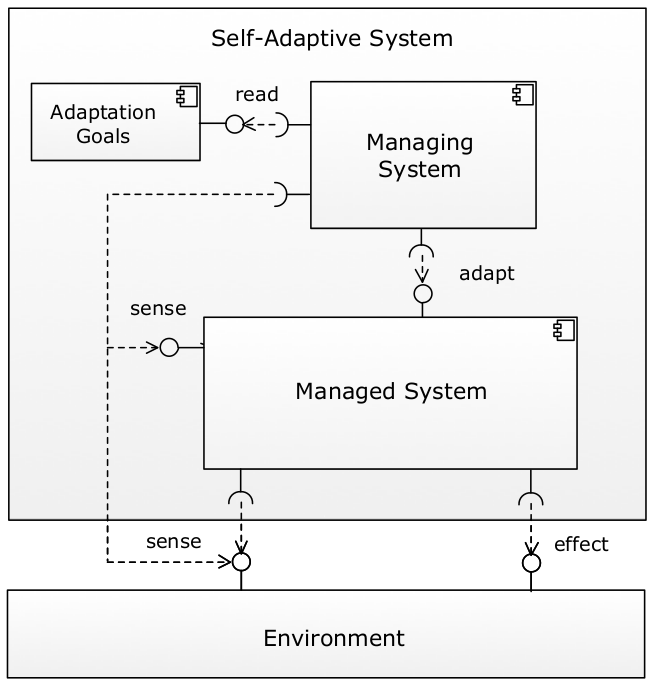
\includegraphics[totalheight=6cm]{figures/conceptualModel}
    \caption{Conceptual Model \citep{softwareEngineeringSA}}
    \label{fig:conceptualModel}
\end{figure}
\subsection{Conceptual Model} Conceptual model of a self-adaptive system comprises of four basic elements: \emph{environment}, \emph{managed system}, \emph{adaptation goals}, and \emph{managing system}.
\begin{enumerate}
\item \textbf{Environment}. The environment refers to the part of the external world
which the self-adaptive system interacts and in which the effects of
the system will be observed and evaluated. Example: the environment of
a robotic system includes physical entities like obstacles in its path
as well as external cameras and software drivers.
\item \textbf{Managed System}. The managed system comprises the application code that
realises the system's domain functionality. Example: navigation of a
robot and transporting loads is performed by the managed system.
\item \textbf{Adaption Goals}. The adaption goals are concerns of the managing system
over the managed system; they usually relate to the software qualities
of the managed system:
\begin{itemize}
\item \textbf{Example:}
\begin{itemize}
\item Example Problem: New elements need to be integrated in a large
IoT application. Installing, configuring, and integarating
heterogenous elements is time consuming and error prone.
\item Example Solution: Automated integration and configuration of new
elements following high-level policies. The rest of the network
adapts automatically and seamlessly.
\end{itemize}
\end{itemize}
\item \textbf{Managing-System}: The managing system comprises the adaption logic that deals with one or
more adaption goals. Example: a robot may be equipped with a managing
system that allows the robot to adapt its navigation strategy to
ensure a certain number of tasks are performed within a given time
window under changing operation conditions.
\end{enumerate}

\pagebreak
\subsection{Engineering Self-adaptive systems}
        The four elements: Monitor, Analyse, Plan and Execute the basic
		functions of any self-adaptive system. They share common Knowledge.

\begin{figure}[H]
\centering
	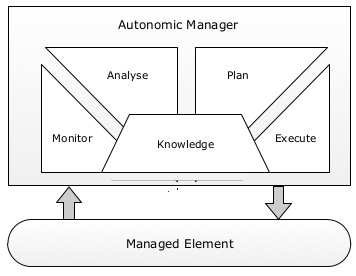
\includegraphics[totalheight=6cm]{figures/mapek}
    \caption{MAPE-K Model \citep{softwareEngineeringSA}}
    \label{fig:mapek}
\end{figure}
\begin{itemize}
           \item \textbf{Monitor}: acquires and processes data from the managed element and
              iTs environment and updated the Knowledge element.
           \item \textbf{Analyse}: uses data from Knowledge element to determine if there is
              a need for adaptation of managed element.
           \item \textbf{Plan}: puts together a plan that consists of one or more adaption
              actions, if an adaptation is needed.
           \item \textbf{Execute}: executes the plan that adapts the managed element as
              needed.
\end{itemize}
\subsubsection{The model based approach  \\\\}
An alternative to using machine learning is ActivFORMS, that uses statistical models.
ActivFORMS (Active FORmal Models for Self-adaptation) is a model-based
approach that provides guarantees for the adaptation goals of self-adaptive systems with some degree of confidence \citep{softwareEngineeringSA}. In ActivFORMS, formally specified
feedback loop models are verified for correctness before deployment and then deployed on top of a virtual machine that directly executes the models to realize
adaptation. ActivFORMS extends the MAPE-K loop with a statistical model
checker that connects with the Analyzer. The statistical model checker supports
the Analyzer with estimating the quality properties that are subject to adapta-
tion for each adaptation option. The statistical model checker uses simulation
and statistical techniques to estimate the quality requirements. The confidence
of the estimated values is dependent on the number of simulations.
\pagebreak

\subsection{Machine Learning concepts \\}
\subsubsection{Definition \\}
Machine learning can be defined as the process of solving a practical problem of solving a practical problem by 1) gathering a dataset, and 2) algorithmically building a statistical model based on that dataset.
\subsubsection{Types of learning \\}
Learning can be supervised, semi-supervised, unsupervised and reinforcement. As far as the scope of this book goes I will discuss only supervised and semi-supervised types of learning.
\begin{itemize}
\item In supervised learning, the dataset is the collection of labelled examples. Each example contains a feature vector (where elements of the vector map to a certain feature like bodyweight, height, etc) and a category (class if you will). The goal is to use that dataset to produce a model that takes an input vector and outputs information that allows deducing the label for this feature vector. For example, the model created using the dataset of pictures of fruits could take as input a feature vector describing a fruit and output what kind of fruit it is. On the other hand the unsupervised learning contains only unlabeled examples.
\item In semi-supervised learning, the dataset contains both labelled and unlabelled. The goal here is the same as with the supervised learning. We hope that using many unlabeled examples can help the learning algorithm to produce a better model. 
\end{itemize}
\subsubsection{Fundamental algorithm types\\}
\begin{itemize}
	\item \textit{Classification} is a supervised learning algorithm that aims at assigning an observation to 
	 a labeled class. Spam detection is a famous example of classification.
	 \item \textit{Regression} if a supervised learning algorithm that aims at predicting the values of dependent variables
	  based on observation. Estimating house price valuation based on house features, such as area,
the number of bedrooms, location and so on is a famous example of regression.
\end{itemize}
\begin{figure}[H]
\centering
\subfigure[Linear Regression for one-dimensional examples \cite{machineLearning}]{\label{fig:energyConsumtion}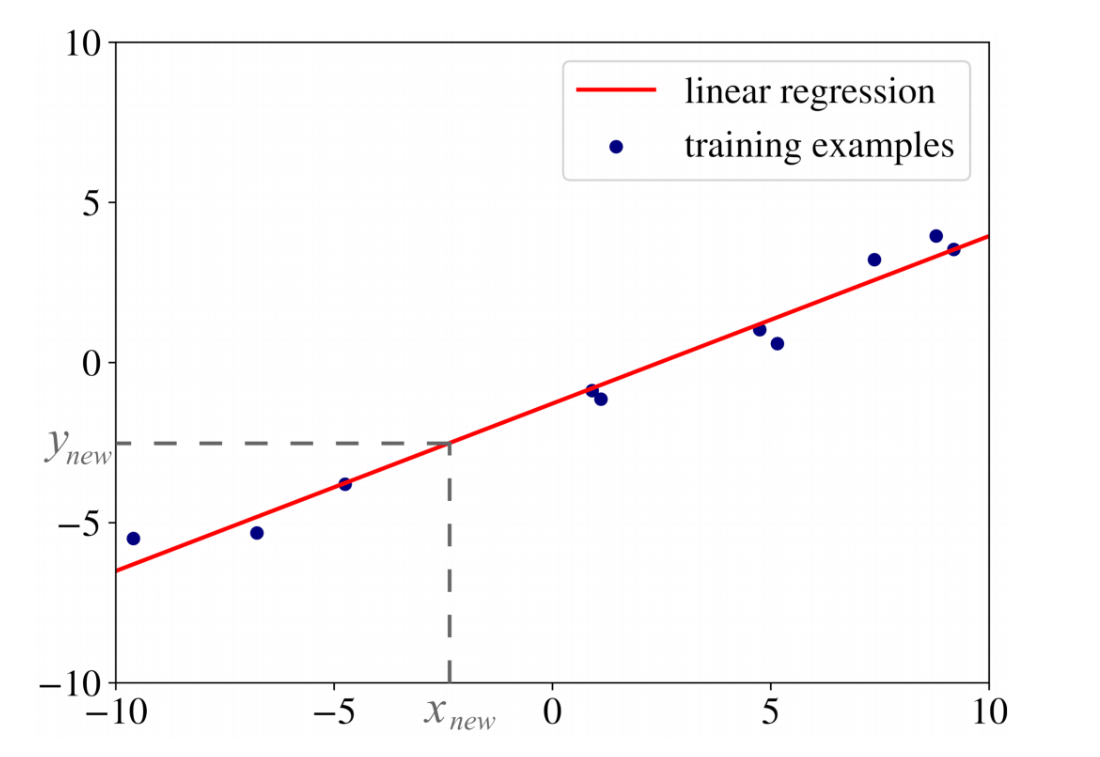
\includegraphics[width=6cm]{figures/linearRegresion}}
\subfigure[Classification model \cite{machineLearning}] {\label{fig:packetLoss}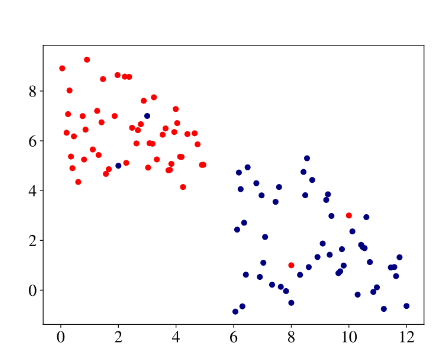
\includegraphics[width=6cm]{figures/classification}}
\end{figure}
\subsubsection{Forms of learning\\}
\begin{itemize}
	\item \textit{Transfer Learning}. In transfer Learning, you pick an existing model trained on some dataset and you adapt this model to predict examples from another dataset, different from the one the model was built on.
	 \item \textit{Online learning}. In online learning data becomes available in a sequential order and is used to update our best predictor for future data at each step, as opposed to batch learning techniques which generate the best predictor by learning on the entire training data set at once. Online learning algorithms may be prone to catastrophic interference where the model forgets past learned examples, a problem that can be addressed by incremental learning approaches.
	 \item \textit{Incremental learning}. In Incremental learning input data is continuously used to extend the existing model's knowledge i.e. to further train the model. It represents a dynamic technique of supervised learning and unsupervised learning that can be applied when training data becomes available gradually over time or its size is out of system memory limits.
\end{itemize}
\subsubsection{Some pitfalls\\}
Common problems with machine learning are underfitting/overfitting models. These problems are usually caused by the training data containing errors/noise. Therefore it is very important that the learning algorithm is trained using good quality data.  
\begin{figure}[H]
\centering
	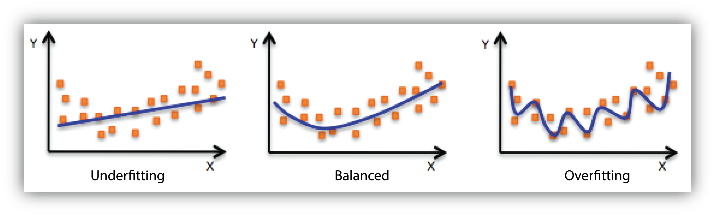
\includegraphics[totalheight=4cm]{figures/fitness2}
    \caption{Fitness of a model \cite{machineLearning}}
    \label{fig:fitness}
\end{figure}

{\footnotesize The definitions for Machine learning were taken from \cite{machineLearning}}
\section{Applying machine learning techniques to self-adaptive systems}\label{sec:p2}
This section is dedicated to machine learning methods that can be used to optimize SAS. \\
 The current research focuses on integrating an online learning module within the MAPE-K model, specifically to the \textbf{Analyzer} and \textbf{Planner} modules.  Some methods do not rely only on the MAPE-K module to perform, they have also a preprocessing phase that typically happens offline, such as in \cite{transferLearning} where using Simulations and transfer learning enables the online learner to make better decisions. During the pre-processing phase the system gathers data in order to train a learning algorithm. This time can take one week or more.\\ 
The evaluation of such algorithms is typically performed on real world systems such as IoT systems like DeltaIoT, or Robotic systems navigating through a terrain, or highly configurable systems like CloudRM, BerkeleyC, BerkeleyJ, LLVM.\\
 \cite{decisionMakingSASystems} presents a method for taking costs into account defined by stake holders when building SAS. Certain adaptions can result in degrading of the system despite seeming an optimal choice to the adaptive algorithm.\\

\subsection{Reducing Search Space using an online learner method}
This method from a paper by Danny Wayns and other collegues \citep{efficientAnalysisAdaptionSpaces} introduces a incremental learning algorithm with the goal of reducing the adaption space. Less adaption option to explore would mean faster converge time and training time. The main idea is that not all configuration are are important, by finding pareto-optimal configurations, an accurate model is still able to be build. This is also  demostrated to be empirically true on the paper by P.Jamshidi  \cite{SAAutoRobots}.
The paper by D.Wayns \cite{efficientAnalysisAdaptionSpaces} takes the challenge on a IoT system. 
Tested on DeltaIoT IoT system which contains a set of 37 motes deployed on a campus. Each Mote is equipped with
RFID, passive infrared and heat sensors that collects data that it relays to the gateway using wireless 
multi-hop and time synchronized communication. Commucation is organized in cycles of 12  minutes with slots. Each slot defines
a send and receiver mote. The motes are battery powered and sending messages costs the most energy.
The sensor data are forwarded to an end user application to monitor
campus area and take action when needed. The total number of adaption options for this system is \textbf{4096}
\\
The uncertainties considered are \textit{network interference} and \textit{fluctuating load of messages}
The adaption goals are:
\begin{itemize}
	\item The average packet loss over 12 hours should not exceed 10\% of the messages sent
	\item The average latency over 12 hours should not exceed 5\% of the cycle time
	\item The average energy consumtion over 12 hours should be minimized
\end{itemize}
\subsubsection{Implementation \\\\}
\begin{figure}[H]
\centering
	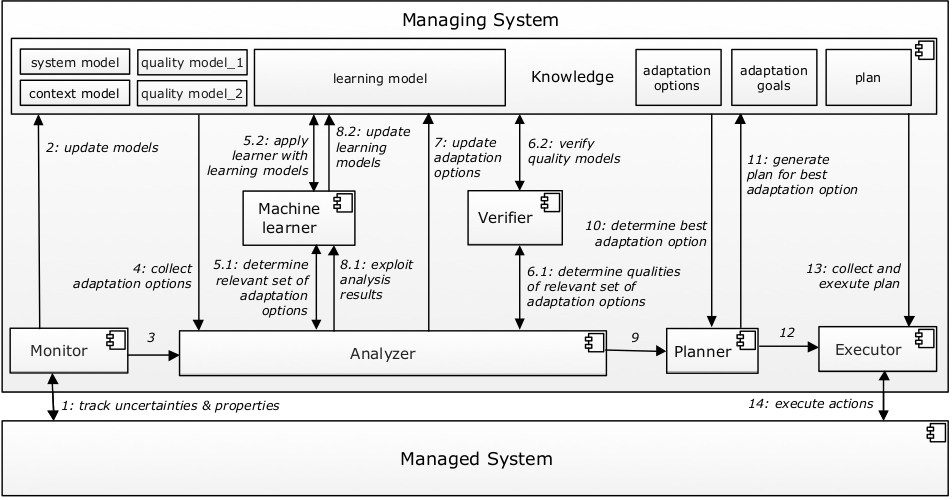
\includegraphics[totalheight=6cm]{figures/mLearner}
    \caption{MAPE-K with Machine Learner \cite{efficientAnalysisAdaptionSpaces}}
    \label{fig:mlearner}
\end{figure}
Attached to the \textit{Analyzer} is a Machine learner Module that determines a set of relevant adaption options.
It comprises of a learning algorithm and a model. The model comprises of a target function that we want to learn.
It allows mapping adaption options to classes, weather it complies with adaption goal or not. Once done it triggers
the \textit{Verifier} which checks the adaption options choosen and returns result back to \textit{Analyzer} which trains
the machine learning algorithm with new results, continuing the learning process and improving the model. 
\\
The algorithm is implemented using a classification and regression incremental learning algorithm. 
An alternative to online learning would \textit{batch learning} which implies the module learns with the whole collection of data. However an exponential adaption space would pose a serious bottleneck and training data may not be available at design time. On a paper \citep{allVSOne} where \textit{incremental learning} is put up to test with its counterpart \textit{retrained learning} it is shown empirically that \textit{incremental learning}:
\begin{itemize}
\item achieves better accuracy under certain conditions
\item leads to faster training time
\end{itemize}
The paper \cite{allVSOne} shows that incremental learning trades off accuracy for faster training time, but in practice the differences are trivial and the system would certainly benefit from faster training time. 

\subsubsection{Results\\\\} 
\begin{figure}[H]
\centering
	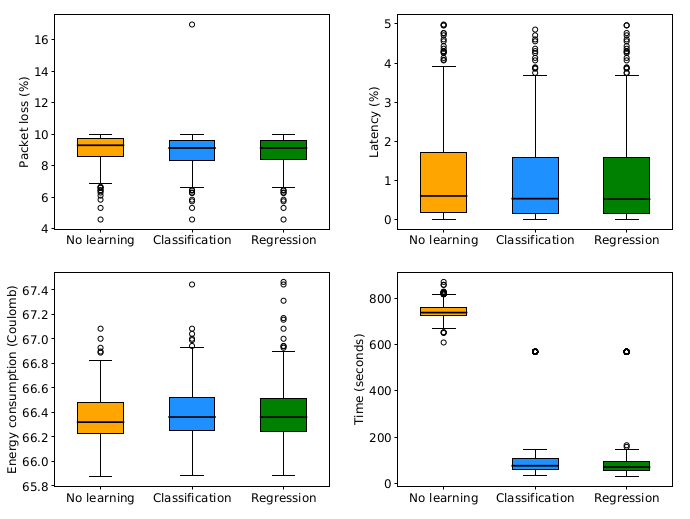
\includegraphics[totalheight=8cm]{figures/resultsMLearner}
    \caption{Adaptation results with and without learning \citep{efficientAnalysisAdaptionSpaces}}
    \label{fig:resultsMLearner}
\end{figure}
The results show that the adaption space can be reduced  significally, in this case by 75\%, with machine learning
without affecting the realization of adaption goals.

\subsection{Evolutionary aware algorithm using the feature model}
In the paper \cite{featureModelGuidedLearning}, another online learning method is proposed using a feature model method \textbf{Feature Model}. 
\textit{A feature model} is a tree or a directed asyclic graph of features. Each Feature can be decomposed into
\textit{mandatory}, \textit{optional} or \textit{optional} sub-features. Using constrains such as \textbf{exludes}
or \textbf{requires} we can express inter-feature depedencies. Using \textit{Feature deltas} which are just changes 
in the feature model before and after an evolutionary step we can capture changes to the adaption space due to evolution. We are still using an online learner like in the first method we discussed but now we guide it on which features to explore first. We can explore the new features added by evolution first or use \textbf{the feature degree strategy} which make an informed decision on which of the feature to explore first by introducing the notion of \textbf{a feature degree} which is the number of feature combinations that contain a feature \textit{f}, as there is a higher probability to of finding an effective feature combination when considering features with high degree.

\begin{figure}[H]
\centering
	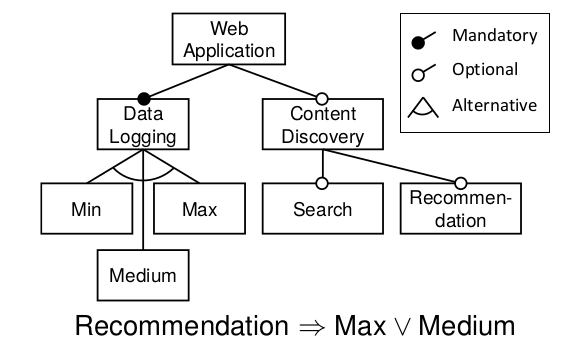
\includegraphics[totalheight=6cm]{figures/featureModel}
    \caption{Feature Model of Self-Adaptive web application \cite{featureModelGuidedLearning}}
    \label{fig:featureModel}
\end{figure}
The paper introduces \textit{an evolutionary aware modified incremental algorithm}.
It is tested against the random version on CloudRM, BerkeleyC, BerkeleyJ, LLVM systems.

\subsubsection{Results \\\\}
As shown in figure \ref{fig:featureModelResults}
We can achieve on average 65\% reduction of explored feature combination in a dynamic adaption space setting. 
However the evolutionary aware feature degree strategy does not show any significant improvement over the evolutionary aware random version, which raises the question why. The paper argues that first exploring
feature combinations added by evolution and exploiting
knowledge about whether a feature was part of an effective
feature combination in the past has a stronger impact on
convergence than how the adaptation space is traversed. I would argue that EvoRand would be an unpredictable way of implementing the algorithm as incomming features are totally random. The results here might deceive us and actually using the feature degree version could deliver more reliable results. In the end I would say that imposing a structure on the adaption space and using a reliable metric such as a feature degree allows the online learning algorithm to make better decisions. 
\begin{figure}[H]
\centering
	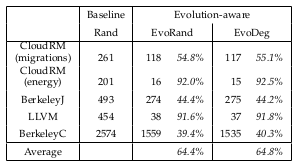
\includegraphics[totalheight=6cm]{figures/featureModelResults}
    \caption{Cumulative number of feature combinations ex-
plored during system evolution and reduction (in \%) com-
pared with baseline. \cite{featureModelGuidedLearning}}
    \label{fig:featureModelResults}
\end{figure}

\subsection{Training the model using simulations and transfer learning method}
The method introduced in the paper \cite{transferLearning} shows a 
The main idea is to learn the model using cheap samples based on a cost function on design time then incorporate the model on a MAPE-K loop using transfer learning using a \textit{kernel function} and in our case a \textit{Gaussian Process Model (GP Model)} which is a framework that reasons using mean estimates and confidence intervals. The GP allows us to capture the relatedness between input configuration and the kernel function allows us to capture the relatedness between the the sources. The effectiveness of a transfer learning algorithm depends on the source environment and how it relates to the target. If the relation is strong and the transfer learning can take advantage of it, the performance in the target prediction can significantly improve. The paper \citep{transferLearning} presents this solution in different settings such as a \textit{robotic system} and a \textit{stream processing system}. 
\begin{figure}[H]
\centering
	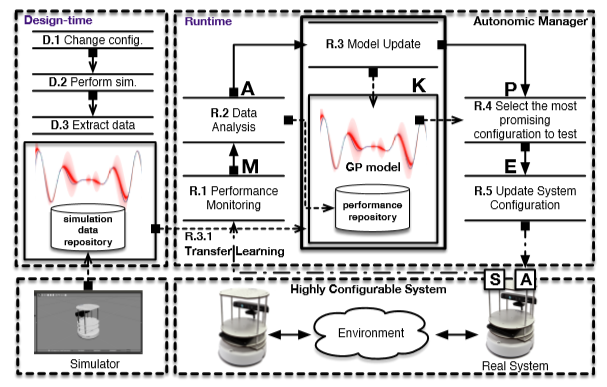
\includegraphics[totalheight=8cm]{figures/transferlearning}
    \caption{Integrating transfer learning with MAPE-K loop \cite{transferLearning}}
    \label{fig:transferlearning}
\end{figure}

\subsubsection{Observations\\\\}
The results backed up by empirical data gathered tell us that, we can indeed learn a fairly accurate model with only a few numbers of samples from target environment and the samples from source environment are cheaper. Using larger samples reduces the variance of prediction error. The training time increases monotonically when increasing the size of sample size. However the relatedness is an important factor to keep in mind and since the tests done in the paper are carried under the assumption that the source environment and target environment are related to a certain degree, the reality might be different. Finding or building a relating system is not without its costs, and some SAS might be better suited for transfer learning than other. Take for example, a SAS that needs to be protected against malicious attacts. Finding a relating environment for such a system might be more complex than a path finding robotic system. All in all, we can positively say that this approach is a viable way to improve prediction accuracy.

\subsection{A cost-benefit analysis method}
Costs of adaption are often neglected because there is not a straight forward path on how to do it, and there is little research going on for it. Sometimes the costs of adapting are high, to have any benefit at all \citep{toAdaptNotToAdapt}.
 The paper \cite{decisionMakingSASystems}  presents with CB@R (Cost Benefit analysis at Runtime). It takes its ideas from CBAM which is already an established method for analysing the costs and benefits of architectural designs of software systems. It allows the stakeholders to choose among different architectural designs based on their VFC (Value For Cost). In contrast to CBAM, CB@R is an automated approach that makes architectural reconfiguration decisions of the system at runtime to deal with uncertainties. A set of runtime models maintained in
the Knowledge repository is required. The models include a
\textit{system model} that provides an abstraction of the managed system relevant to
realize the adaptation goals, and a \textit{context model} that provides an abstraction
of the relevant parts of the environment in which the system operates. To determine the benefits of adaption with CB@R a set of \textit{utility response curve models} are required, one for each quality property that is subject of adaption.  They are defined in consultation with the stakeholders and express how the utility for different values of the quality property changes as valued by the stakeholders.\\
This approach requires also a cost model that represents various implecations of realising adaption, such as delay caused through adaption, resources required, etc. The cost model should allow determining the cost for
each adaptation option, so that CB@R can perform a cost-benefit analysis for
the different adaptation options.
  \begin{figure}[H]
\centering
	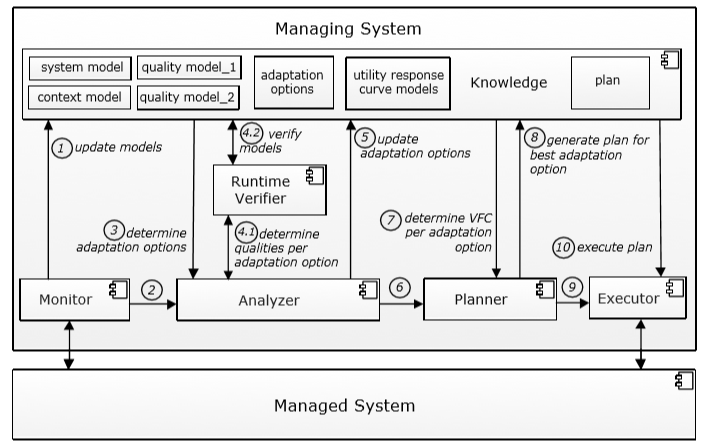
\includegraphics[totalheight=6cm]{figures/cb@r}
    \caption{MAPE feedback loop with runtime decision-making using CB@R \cite{decisionMakingSASystems}}
    \label{fig:cb@r}
\end{figure}
\subsubsection{Realisation \\\\}
The MAPE elements exploit the runtime models to realise CB@R as follows. The
Monitor tracks quality properties and uncertainty parameters of the managed
system and the environment. The collected data is used to update the system
model, the context model, and the different quality models. When the Analyzer is triggered it determines the adaptation options, i.e., all relevant
configurations of the managed system that can be reached through adaptation
from the current configuration. For each adaptation option, the Analyzer determines the expected qualities that are relevant for adaptation using the Runtime
Verifier. To that end, the verifier uses the runtime models of the different
qualities, possibly combined with the system and context models, and computes
estimates for the different qualities of each adaptation option. The verification results, i.e., the expected values of the quality properties associated with the
different adaption options, are then updated in the Knowledge repository.
Next, the Planner determines the Value For Cost (VFC) for each adaptation option. To calculate the total benefit of an adaptation option the
Planner first computes the utility for each quality. To that end, the Planner uses
the estimates for each quality as determined by the Analyzer. The Planner determines the utility for each estimated quality property using the utility response. Effective Decision Making in Self-Adaptive Systems
curves model for the quality. This is repeated for each quality that is subject to
adaptation. As different quality attributes will have different importance to the
stakeholders, each quality is assigned a weight (the weights express the relative
importance of a qualities, so the sum of the weights should be equal to one).\\
\begin{equation}
 VFC = \frac{Benefit}{Cost} 
 \end{equation}
 The CB@R does not use machine learning techniques but rather statistical models. In combination with an online learner it can enhance the machine learner with it's cost-benefit analysis and the make better decisions as to what adaption option is better suited for adaption in a given situation.
\subsubsection{Results \\\\}
This approach is evaluated on the same DeltaIoT system discussed previously. For evaluation the model is compared against a rule based model and a reference model (VersaSense). Without going into much technical detail, the results in the paper show us:
 \begin{figure}[H]
\centering
\subfigure[Results: energy consumtion \cite{decisionMakingSASystems}]{\label{fig:energyConsumtion}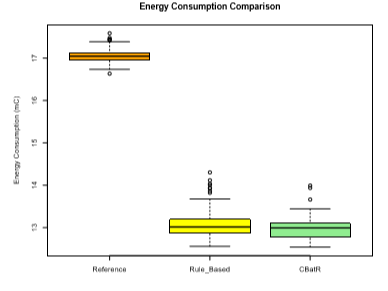
\includegraphics[width=6cm]{figures/energyConsumtion}}
\subfigure[Results: packetLoss \cite{decisionMakingSASystems}] {\label{fig:packetLoss}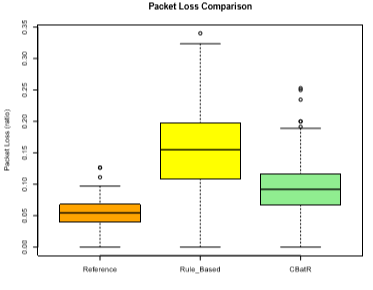
\includegraphics[width=6cm]{figures/packetLoss}}
\end{figure}
	
For energy consumtion both self adaptive approaches are better than the reference model. However for packet loss its obvious that CB@R is able to complete the requirement while the rule base version did not. These results show that substantial benefits can be gained by applying the CB@R method. 

\section{Conclusions}\label{sec:conclusions}
This paper discussed machine learning approaches that outperformed many of the state of the art rule based and conservative approaches on SAS.
\subsection {Comparisson of the methods}
\subsubsection{ActivFORMS: \\}
\begin{itemize}
\item uses statistical models, no need for trainning a model.
\item is not aware of change.
\item predictions are rather probabilistic.
\end{itemize}
\subsubsection{Using an incremental algorithm: \\}
\begin{itemize}
\item The model learns online and can adapt to change by using the incremental learner.
\item The decisions made by the online learner do not take costs of adapting into account which might be negative to have any benefit from the adaption.
\item A new hyperparameter is needed to use the incremental learner \textit{batch size}. Depending on it the incremental learner can learn better or worse.
\end{itemize}
\subsubsection{Feature model method: \\}
\begin{itemize}
\item The model learns online and can adapt to change better by using an evolutionary aware algorithm.
\item Still the costs of adaption are not taken into account.
\end{itemize}
\subsubsection{Transfer learning: \\}
\begin{itemize}
\item Makes better decisions using models trained in simulatons where the cost of training is low. 
\item The result depend on the relatedness of source environments. The more related the source enviromnemnt the better the results. 
\end{itemize}
\subsubsection{CB@R: \\}
\begin{itemize}
\item Allows for a cost-benefit analysis of system on runtime. 
\item Can be used in combination with an online learner module and enhance it's performance. 
\end{itemize}
\nocite{*}
\bibliography{template}

\end{document}
